%%%%%%%%%%%%%%%%%%%%%%%%%%%%%%%%%%%
\chapter{Progress}

This chapter exposes the work done until now in the project. It will focus on the choices I have made, the stages of developpment and the questions remaining. All the codes are available on the Github repository of the project.


\section{Data Exploration}

As the main dataset, we use the simulation results on an unstructured mesh of measurements with a very high density in the low middle part of the space. The simulation used has $100'040$ points over $988$ timestamps. For the purpose of testing our codes and algorithms,  we are going to use subset of the whole dataset containing a few hundreds to a few thousands of points. I have made the choice to first use a subset of the whole dataset containing $2'488$ point and created by cropping the space to a cube of $30\times30\times30\times$ at the center of the original space. 


 Several fields are present in the simulation : the \textbf{pressure}, the \textbf{tracer} concentration, the \textbf{background tracer} concentration and the \textbf{velocity}. We represent in the next figures, two cuts made to visualise the tracer and the tracer background. \\ 

The \textbf{tracer} represents the propagation of a pollutant generated from the centre of the domain at ground level. It aims a representing a busy intersection. \\

The \textbf{background tracer} represents pollution waves common in urban environment. Its characteristic generation equation is periodic and given by : 

\begin{equation}
	C(t)= \frac{1}{2} \left( \sin \left( \frac{2\pi t}{T} \right) + 1 \right)
\end{equation}



As we can see by observing the time propagation of those fields,  the wind is pushing the pollutants in a certain direction. Because of this, be observe that the \textbf{tracer} concentration is mainly visible downwind, in contrast of the \textbf{background tracer} which has visible propagation over the whole space. We can therefore already deduce that the \textbf{background tracer} contains much more information and should be used for optimising the sensor positions. 


\section{Implementation}

In this section I will quickly review the functionalities that I have implemented and that are working to this day. I relied on Python 3.7, various libraries that I ran my code on the cluster of the DSI.  \\

\subsection{Initialisation}
The raw data is contained in VTK files. I have implemented functions in python that allows the importation, the cropping of the space, the extraction of the fields and interest and the location of the points and the saving in files for making quicker the loading procedure. 

\subsection{Modeling}

I have implemented the full GP training and estimation directly using numpy. It this implementation I have chosen to use a kernel with arbitrary parameters in order to test the accuracy of the optimisation. \\

After this I have used the GPy library \citep{gpy_gpy:_2014} for its full GP implementation and its hyper-parameters optimisation functionalities. The kernel parameters here were optimised using the integrated methods and the model was trained on the full subset of data. \\

I have also implemented using GPy library a spare GP modelisation. GPy includes an optimised implementation of the \textbf{VFE} sparse GP. It enables the optimisation of the variational parameters and the hyper-parameters such as the position of the inducing points. 

\subsection{Optimisation}

I have used the previously trained GPs models in the algorithms described earlier. I have implemented in python two of the proposed optimisation algorithms. The naive greedy approach (algorithm \ref{alg:greedy} ). \\
The Lazy approach developed using python heaps. (algorithm \ref{alg:lazy}). This version is as expected much faster than the standard version.  \\ 

For illustration we plot in the following figure \ref{fig:k10_fullGP_results} the results obtained with full GP of a small subset of the space described earlier for a number of sensors $k=10$.  On this subspace, I have made the choice to compute an isotropic covariance matrix (Exponential kernel,  Matern 3/2 and 5/2) with a length-scale of $l=3$ for testing the performance of the optimisation algorithm. The sensors optimal positions are marked in red.  



\subsection{Display and Exportation}

In order to visualise the results of the optimisation, I have implemented function that saves the optimal locations in VTK files for an easier visualisation. I have also implemented function enabling visualisation with matplotlib of sections of the space. 

\section{Discussion}

In this section, I will try to show and justify the approach I have taken, as well as the remaining questions and problems to be solved. 

\subsection{Summary of the GP Sensor Optimisation}

The methods developed by \citet{krause_near-optimal_2008} are using the full Gaussian process in to greedily place sensors. The algorithm consists in the estimation of the best “new” sensor to add the set of existing sensor based on a mutual information gain criterion. This criterion can be computed with two Gaussian processes. One that estimates the covariance of the sensor candidate $y$ given the set of previously selected sensors $\A$ : $K_{y | \A}$. The other GP allows the computation of the covariance of the candidate $y$ given the rest of the locations in the space $\bar{\A} = \V \backslash ( \A \cup y )$ : $K_{y | \bar{\A}}$. We recall the problem that is to be solved is :

\begin{equation}
    y^* = {\arg \max}_{y \in \S \backslash A } \: \frac{K_{y | \A}}{K_{y | \bar{\A}}}
\end{equation}

This has to be computed theoretically for every candidate point of the dataset, and this for every sensor we add to A. The naive version is described in \ref{alg:greedy} and a lazy version of the algorithm is available at algorithm \ref{alg:lazy}.

\subsection{Covariance Estimation}

The GP estimation of the conditional covariances mentioned previously relies heavily on the initial joint covariance. 

\begin{equation}
    K_{y | \A} = K_{yy} - K_{y\A} K_{\A\A}^{-1} K_{\A y} \label{equ:cond_cov}
\end{equation}

This is why it is really important to have a proper way to estimate the covariance in our space of interest. 

Those are the three main approaches I have identified initially. 

\begin{enumerate}
    \item Use the sample covariance of the given data
    \item Use a non-stationary covariance that we learn with the data
    \item Use isotropic and stationary covariance and learn its parameters with the GP optimisation. 
\end{enumerate}

\subsubsection{Sample Covariance}
First, the use of the sample covariance as an estimator of the true covariance has proven not to work. The resulting covariance is singular and therefore can't be inverted for the use in \ref{equ:cond_cov}. Also, it is, in general, a poor estimator of the real covariance when the number of points is much larger than the number of samples. The memory needs to store such a full matrix is also not practical as on the cluster it used almost 75\% of all the memory. \\

\subsubsection{Non-Stationary Covariance}

Secondly, the use of non-stationary covariance estimator as suggested by \citet{krause_near-optimal_2008} is probably the best solution for our problem.

Several approaches have been developed in the literature about this specific subject. Many methods were design in the Geostatistical field where the main application is the interpolation a small number of sensor points to the whole space (kriging). 

There are also interesting studies on the estimation of sparse covariance matrixes. \\

\todo{Explain that I use the VFE only for predicting the canditate given the whole dataset. The other GP is tracktable because it is conditioned by the number of sensors already placed.}


%
%But the approach we need to have is quite different from the one they present. There are main differences : 
%
%\begin{itemize}
%    \item The data that they have is not a simulation with a very small time step. They are dealing with daily/hourly observations and not with steps of 30s as we have.      
%    \item They don't have a very dense network of sensors and are not ?? Relevant ??
%    \item Scalability. Not talking of hundreds of sensors, but 100000 points to explore. (not for covariance)
%\end{itemize}


%Propagation data ? very different ? 

\subsubsection{Isotropic Covariance}

For now, I have decided to keep the kernel stationary and isotropic  in order to focus on the scalability of the GPs and the algorithm. The main advantage of this kind of covariance is that is relies uniquely on parameters that can be optimised in the training of the GP, whereas data-driven covariance requires much more memory and computation. 

\subsection{Gaussian Process}

Initially I implemented the full GP version proposed in the paper of \cite{krause_near-optimal_2008}. For a small dataset it gives consistent results. \\

I have then explored ways of making GPs more scalable and focused on the VFE sparse Gaussian Process. For larger datasets I am able to optimise the hyperpameters and the positions of the induction points before using this model.  \\

I use the sparse GP 

\section{Implementation Details}

\subsection{Environment}

For this project the code was implemented using \textit{python 3.7} and the following list of libraries : 

\begin{itemize}
	\item numpy
	\item pandas
	\item matplotlib
	\item GPy
\end{itemize}

\todo{Update the list of packages using conda}
\todo{Make a table with the version number}

\subsection{Initialisation}

\todo{This is a copy paste of the previous section Initialisation section}

\paragraph{Data Preprocessing}

\todo{Update paragraph with new preprocessing}
In order to make the data usable for the rest of the project we apply some preprocessing of the previously selected dataset. \\

First we analyse the quantity of zero elements present in the data \textbf{in function of the time}. We count every point of data that has a value over $\tau = 10^{-4}$. This gives us the plot of figure \ref{fig:sumtime}. As we can see, it takes some initial time for the tracer to propagate to some kind of steady state, at around 33\% of the points. This is why we decide to use only the part of the data where the tracer concentration is steady across the space : we choose to cut the first 200 samples of the data (100s). \\

\begin{figure}[]
\centering
	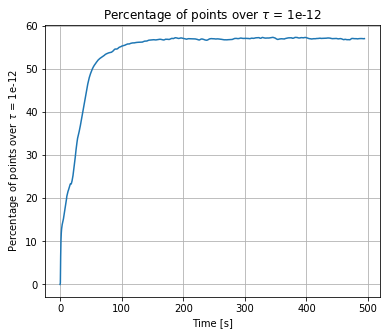
\includegraphics[width = 0.7 \textwidth]{figures/DataAnalysis/SumDataTime}
	\caption{Percentage of significant points in function of the time for $\tau = 10^{-4}$}
	\label{fig:sumtime}
\end{figure}


Furthermore, we decide to \textbf{round to zero} the values that are smaller than the previous threshold of $\tau = 10^{-4}$. This can be motivated by the fact that it will allow to use the sparsity of the data to make the algorithm faster. This means that we will approximatively set a 66\% of the tracer values to zero.\\

We try to find a trend in the data that we could exploit in the rest of the project. We plot for example the mean tracer value for each location in function to the distance to the origin of the tracer. This scatter plot can be seen on figure \ref{fig:tracerdistance}. 

\begin{figure}[]
\centering
	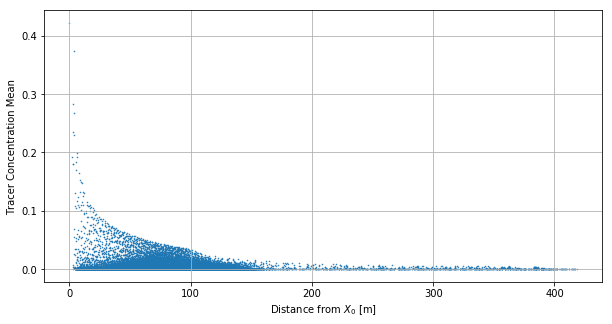
\includegraphics[width = 0.7 \textwidth]{figures/DataAnalysis/TracerMeanDistance}
	\caption{Mean value for each point in function of the distance to the tracer's origin}
	\label{fig:tracerdistance}
\end{figure}


As we can see there is no immediate trend that can be detected, so we proceed to a \textbf{centering of the Data} that will enable a faster processing of the covariance matrix. 












